\documentclass[11pt, oneside, titlepage]{article}
\usepackage{fancyhdr}
\usepackage{graphicx}
\usepackage{imakeidx}
\usepackage{makeidx}
\usepackage{mathtools}
\usepackage[spanish]{babel}
\usepackage{graphicx}
\usepackage{dsfont}
 
\title{\textbf{Física}\\ Universidad Católica de Ávila}
\author{Francisco Javier Balón Aguilar}
\date{Febrero 2019}

\begin{document}
\maketitle
% Índice de contenidos
\tableofcontents
\newpage

\section{Introducción a la física}
La física es la parte de las \emph{ciencias naturales} que estudia los fenómenos de la Naturaleza con su máxima generalidad. Un fenómeno natural es cualquier cambio que se produce en la Naturaleza. La Naturaleza, a un nivel ontológico, se compone de \emph{cosas, propiedades y relaciones}:

\begin{center}Una pluma (\emph{cosa}) azul (\emph{propiedad}) escribe sonbre papel (\emph{relación entre pluma y papel}).\end{center}

\subsection{Fenómenos físicos}
En las ciencias naturales puede haber fenómenos físicos, químicos (composición de sustancias) y biológicos (aspectos vitales). 

\subsubsection{Magnitudes físicas}
Todo fenómeno natural es discernible por nosotros gracias a que las propiedades de las cosas varían, se diferencian unas de otras. Esta diferencia es en la cantidad o en la forma. Así llegamos al concepto de magnitud física.

Una magnitud física es una propiedad de un objeto cuantificada numéricamente, es decir se relaciona de forma unívoca la propiedad y el número. Para que sea realmente univoco debemos añadir una unidad.

Dada una cantidad de una magnitud física que queremos medir ($A$), y sea una cantidad determinada de esa magnitud física que tomamos ($A_0$), entonces la cantidad dada se expresa como un número ($n = (A)/(A_0)$), dónde $n \in \mathds{R}$. Así pues:
\[
(A) = n(A)_0
\]

Existen dos tipos de magnitudes físicas:
\begin{enumerate}
\item \emph{Magnitud fundamental}. Es aquella magnitud física que no se define a partir de otras.
\item \emph{Magnitud derivada}. Es aquella que se define a partir de magnitudes fundamentales.
\end{enumerate}

\subsubsection{Sistema de unidades}
Los sistemas de unidades y sus correspondientes magnitudes determinan las \emph{unidades}, y por tanto magnitudes, que debemos tomar como \textbf{fundamentales}.

El sistema generalmente usado y recomendado es el \emph{Sistema Internacional (SI)}:

\begin{center}\begin{tabular}{llr}
	\textbf{Magnitud física} & \textbf{Unidad} & \textbf{Abreviatura}\\
	Longitud & Metro & $m$\\
	Masa & Kilogramo & $kg$\\
	Tiempo & Segundo & $s$\\
	Corriente eléctrica & Amperio & $A$\\
	Temperatura & Kelvin & $K$\\
	Intensidad luminosa & Candela & $cd$ \\
	Cantidad de sustancia & Mol & $mol$\\
\end{tabular}\end{center}

El sistema \emph{cgs} (\emph{centímetro, grado, segundo}) utiliza unidades que son submúltiplos del \emph{SI}. Así el centímetro es 1/100 de metro y el gramo es 1/1000 de kilógramo. Utiliza además, algo común en física, prefijos para determinar las magnitudes, así:

\begin{center}\begin{tabular}{lcr}
	\textbf{Factor} & \textbf{Prefijo} & \textbf{Símbolo}\\
	$10^{24}$ & yotta & $Y$\\
	$10^{21}$ & zetta & $Z$\\
	$10^{18}$ & exa & $E$\\
	$10^{15}$ & peta & $P$\\
	$10^{12}$ & tera & $T$\\
	$10^9$ & giga & $G$\\
	$10^6$ & mega & $M$\\
	$10^3$ & kilo & $k$\\
	$10^2$ & hecto & $h$\\
	$10^1$ & deca & $da$\\
	$10^{-1}$ & deci & $d$\\
	$10^{-2}$ & centi & $c$\\
	$10^{-3}$ & mili & $m$\\
	$10^{-6}$ & micro & $\mu$\\
	$10^{-9}$ & nano & $n$\\
	$10^{-12}$ & pico & $p$\\
	$10^{-15}$ & femto & $f$\\
	$10^{-18}$ & atto & $a$\\
	$10^{-21}$ & zepto & $z$\\
	$10^{-24}$ & yocto & $y$\\
\end{tabular}\end{center}

Y el sistema técnico de unidades utiliza el mismo número de unidades que el \emph{SI} o el \emph{cgs}, pero en lugar de la unidad de masa como fundamental, utiliza la unidad de fuerza, el \emph{kilopondio} ($kp$).

\subsection{Divisisón de la Física}
Toda ciencia tiene su objeto. En el caso de la Física el objeto es el estudio de la Naturaleza de la forma más general posible. Así, la Física se divide en teorías físicas, que estudian un aspecto particular de la Naturaleza o desde un pounto de vista concreto. Así:

La Fisica se divide ampliamente en Física Clásica (Física Newtoniana, Electromagnetismo y Teoría de la Relatividad de Einstein) y Física Cuántica (Mecánica Cuántica Relativista y Mecánica Cuántica no Relativista).

En la Física existen diversas constantes universales, que son números simbólicos que determinan una magnitud que no cambia o varía. Las dos más importantes en este caso son la velocidad de la luz ($c = 299\ 792\ 458 m/s$) y la constante de Planck ($h = 6.626070150(69) \times 10^{-34}\ j \times s$). Fijándonos en ambas constantes, las teorías físicas se agrupan en cuatro grandes campos:

\begin{enumerate}
\item \emph{Física Newtoniana}. Comprende la mayor parte de los fenómenos físicos a los que estamos acostrumbrados a ver en nuestra vida cotidiana.
\[v << c \] \begin{center}y\end{center} \[ \Delta E \Delta t >> h\]
Es decir, si en los fenómenos involucrados las velocidades son muy pequeñas comparadas con la velocidad de la luz ($c$) y las acciones (energía por el tiempo) son mucho mayores que la constante de Planck ($h$).
\item \emph{Física Relativista}. Engloba la Teoría de la Relatividad Especial y la Teoría de la Relatividad General de Einstein.
\[v \approx c\] \begin{center} y \end{center} \[\Delta E \Delta t >> h\]
Es decir, si en los fenómenos involucrados las velocidades ($v$) son comparables a la velocidad de la luz ($c$) y las acciones son mucho mayores a la constante de Planck ($h$).
\item \emph{Física Cuántica no Relativista}. Engloba los fenómenos químicos entre átomos.
\[v << c\] \begin{center} y \end{center} \[\Delta E \Delta t \approx h\]
Es decir, las velocidades ($v$) involucradas son muy pequeñas comparadas a la velocidad de la luz ($c$) y las acciones son comparables a la constante de Planck ($h$).
\item \emph{Física Cuántica Relativista}. Engloba los fenómenos de los núcleos atómicos y de Física de partículas. Comprende Teorías de Cuerdas y Supercuerdas, de Supersimetría (SUSY) o de Gran Unificación (GUT).
\[v \approx c\] \begin{center} y \end{center} \[\Delta E \Delta t \approx h\]
Es decir, tanto las velocidades ($v$) son comparanles a la velocidad de la luz ($c$) como las acciones son comparables a la constante de Planck ($h$). 
\end{enumerate}

\section{Electrostática}

\subsubsection{La carga eléctrica}
La materia está formada por unos constituyentes fundamentales llamados átomos y estos, a su vez, están compuestos por electrones, protones y neutrones. Los protones y neutrones están muy próximos entre sí y constituyen el núcleo atómico. Los electrones están a gran distancia del núcleo atómico. A su vez, los átomos están entre sí separados por grandes distancias.

\begin{figure}[htp]
\centering
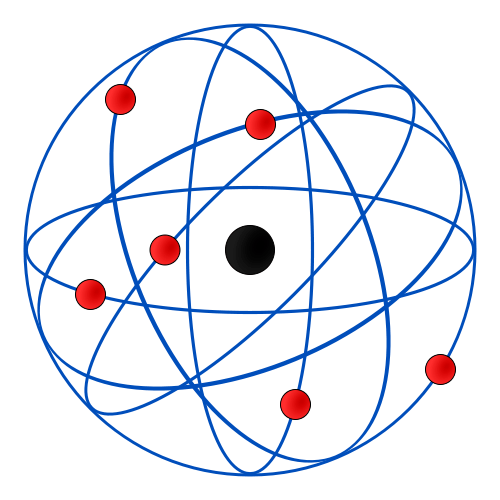
\includegraphics[width=0.3\textwidth]{resources/repatomo.png}
\caption{Representación clásica de átomo.}
\label{}
\end{figure}

Los electrones y los protones tienen una \emph{propiedad intrínseca}, como es la masa en un cuerpo, que es la \emph{carga eléctrica}. Electrones (carga eléctrica negativa) y protones (carga eléctrica positiva) poseen la misma carga pero de signos opuestos (en un átomo la fuerza electrostática ejercida por un electrón, queda anulada por la fuerza electrostática ejercida por un protón.). Los neutrones no poseen carga eléctrica. 

La carga eléctrica se manifiesta a través de la interacción electrostática mediante una fuerza electrostática que repele cargas eléctricas de igual signo, pero atrae cargas eléctricas de distinto signo. 

Como los átomos en la materia ordinaria tienen el mismo número de protones que de electrones, resulta que \emph{la materia ordinaria es eléctricamente neutra}. Cuando por la causa que sea, un cuerpo neutro es abandonado por un cierto número de electrones, habrá en él un exceso de cargas positivas (más protones que electrones), se dice pues que \emph{un cuerpo está cargado positivamente}. Si pasa al contrario, quedan en un cuerpo más electrones que neutrones dando un esceso de cargas negativas, se dice que \emph{un cuerpo está cargado negativamente}.

Los protones son unas 2000 veces más pesados que los electrones. Así en el átomo tenemos cargas negativas muy ligeras (lo que tiene una enorme importancia en aplicaciones prácticas), siendo la carga libre más pequeña que se conoce:

\[
e = 1.60 * 10^{-19} culombios
\]

En \emph{SI} la unidad de carga es el \emph{culombio}. Se define a partir de la intensidad de corriente (\emph{amperio, $A$}), siendo un culombio un amperio por segundo:

\[
[C] = [A*s]
\]

\emph{El principio de conservación de la carga elétrica} dicta que en un sistema aislado la carga se conserva, es decir, la suma de las cargas positivas y negativas en un sistema aislado no varía.

\subsection{Distribuciones de carga eléctrica}
Vamos a tratar con objetos macroscópicos constituidos por millones y millones de átomos. Estos átomos cargados se pueden considerar a efectos macroscópicos como distribuciones continuas de carga.

La cuantificación de la propiedad de la carga eléctrica en este caso se hace como sigue:

\begin{enumerate}
\item \emph{Distribuciones de carga puntuales}. Se supone la carga concentrada en un punto. El llamado punto es un pequeño objeto macroscópico formado por millones y millones de átomos cargados.
\item \emph{Distribuciones continuas de carga}. Son aglomeraciones de carga que, desde el punto de vista macroscópico pueden caracterizarse por densisdades de carga, es decir, la relación entre la suma de todas las cargas que hay en un volumen, superficie o longitud elemental y dicho volumen, superficie o longitud. Pueden ser:
\begin{enumerate}
\item \emph{Densidades de carga volumétricas}.
\[\rho = \lim\limits_{\Delta V \to 0} \frac{\Delta q}{\Delta V}\]
\item \emph{Densidades de carga superficial}.
\[\sigma = \lim\limits_{\Delta S \to 0} \frac{\Delta q}{\Delta S}\]
\item \emph{Densidades de carga lineal}.
\[\lambda = \lim\limits_{\Delta l \to 0} \frac{\Delta q}{\Delta l}\]
\end{enumerate}
Siendo $\Delta q$ la \emph{cantidad de carga} en:
\begin{itemize}
\item $\Delta V$: volumen.
\item $\Delta S$: superficie.
\item $\Delta l$: longitud.
\end{itemize}
\end{enumerate}

\subsection{Ley de Coulomb}
<<La fuerza que actúa sobre una carga puntual fija $q_2$, debido a la presencia de otra carga puntual fija $q_1$, es directamente proporcional al producto de las cargas e inversamente proporcional al cuadrado de la distancia que las separa, está dirigida según la línea definida por ambas cargas, y es respulsiva o atractiva según sean del mismo o distinto nombre las dos cargas.>>

O expresado matemáticamente el módulo de fuerza:

\[
F = K \frac{q_1 q_2}{d^2} 
\]

Dónde:

\begin{itemize}
\item $K$ es la constante de Coulomb. Es dependiente del medio, en el vacío: $K =  9*10^9 Nm^2/c^2$. También se puede expresar:

\[
K = \frac{1}{4 \pi \varepsilon} = 9*10^9 Nm^2/c^2
\]

Dónde:
\begin{itemize}
\item $\varepsilon$ es el coeficiente dieléctrico o permitividad.
\item $\varepsilon$ también es dependiente del medio. Cuando se trate del vacío se denotará por $\varepsilon_0$.
\end{itemize}
\end{itemize}

\subsubsection{El campo eléctrico}
Un campo es un objeto físico, el espacio, con una cierta propiedad, la interacción eléctrica. Es decir, campo es la región del espacio donde se produce un efecto físico caracterizado por una magnitud escalar o vectorial, independiente o no del tiempo.

Así, el campo eléctrico --creado por una carga eléctrica-- es el espacio donde se manifiesta su atracción o repulsión sobre otras cargas.

La intensidad de campo en un punto es la fuerza que actúa sobre la unidad de carga positiva colocada en ese punto, es decir:
\[
\overrightarrow{E}(\overrightarrow{r}) = \frac{\overrightarrow{F}(\overrightarrow{r})}{q}
\]

O, más simplificado:

\[
\overrightarrow{E} = \frac{\overrightarrow{F}_e}{q}
\]

Las líneas de fuerza de un campo electromagnético son las trayectorias que seguiría una carga positiva, sometida a la influencia del campo, en una sucesión de caminos elementales, partiendo, en todos ellos, del reposo.
\begin{figure}[htp]
\centering
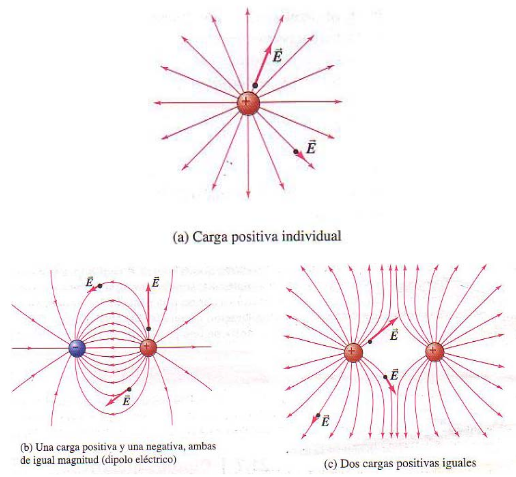
\includegraphics[width=0.8\textwidth]{resources/electrostatica_lineasfuerza.png}
\caption{Ejemplo de líneas de fuerza de un campo electromagnético}
\label{}
\end{figure}

\section{Corriente continua}
Los materiales que existen en la naturaleza pueden ser divididos en \emph{conductores} y \emph{aislantes}, con un grado medio, los \emph{semiconductores}.

En un material \emph{conductor} existen un gran número de cargas que se mueven con libertad en su interior. No son sólo conductores los metales y sus aleaciones, sino los gases ionizados, electrólitos, semiconductores, vacío en la vecindad de un cátodo emisor termoiónico y toda sustancia en que los portadores de carga se muevan con libertad.

La \emph{corriente eléctrica} es la circulación de una carga a través de un conductor. Se llama \emph{conducción} al proceso por el cual la carga se transporta.

\section{Corriente alterna}
\section{Campos magnéticos}
\section{Inducción electromagnética}
\section{Teoría de circuitos}
\section{Electrónica digital}

\end{document}
